\subsection{Problem definition}
A \textit{data stream T} is an infinite time sequence of tuples $T = t_1, t_2, t_3, ...$, with an incremental order such that for two tuples $t_i$ and $t_j$ and $i < j$, denotes that tuple $t_i$ arrives before $t_j$. A tuple $t_i$ consists of the following attributes $t_i = \{ID, TS, A_1, ..., A_m\}$, where $ID$ is an identity attribute to uniquely identify an individual and $TS$ is a timestamp indicating the arrival time of the tuple. In this study the arrival time will be interchangeably used with the term ingestion time, that is the time that a tuple enters the anonymization procedure. Furthermore, let a subset $QID \subset \{A_1, ..., A_m\}$ be the quasi-identifier in the tuple.\\
\\
There are a few assumptions involved in our approach:
1. In line with \citeA{CpppOfDataStreams}, we assume that the attributes $ID$ and $TS$ are not going to be published. 2. The attributes $t_i - QID - \{ID, TS\}$ are not involved in the procedure and therefore can be omitted for the sake of simplicity, however they can just be outputted with the anonymized attributes. 3. While \citeA{CpppOfDataStreams} assume that there possibly are identical $ID$ values, that is, several tuples from the same object, we will assume that each tuple comes from a unique individual. Please note that we had to take this assumption due to technical reasons in the implementation with the Apache Flink framework, since there was no straight forward implementation of non-unique IDs in the processing, however in general our approach can be extended by this feature and for now this assumption does not change the outcome of this study. 4. We assume that the utility of data in stream $T$ is time sensitive, that is, usability of the data decreases with time passed between arrival and release. Without this assumption, that is, if the latency between data arrival and data publishing would be irrelevant, the problem would be trivial. One could simply wait until a batch of data that is large enough to be anonymized (i.e. $k$ tuples) has arrived and thereafter periodically apply a static method to anonymize the data in batches. Furthermore, as described in the previous section, incremental approaches are not appropriate in this problem setting either, because re-publication of the entire data that has arrived up to a certain point in time is highly inefficient and will decrease the utility of the data immensely due to large latency.\\
\\
The $k$-anonymity and $l$-diversity problem, that our algorithm is going to solve can now be defined as follows:
\begin{definition}[$k$-anonymity problem for data streams]
Considering a data stream $T$, an anonymized output stream $T'$ needs to be produced, where every equivalence class that is being released to $T'$ needs to contain at least $k$ indistinguishable tuples with respect to the $QID$.
\end{definition}
\begin{definition}[$l$-diversity problem for data streams]
Considering a data stream $T$, an anonymized output stream $T'$ needs to be produced, where every equivalence class that is being released to $T'$ needs to contain at least  $k$ indistinguishable tuples with respect to the $QID$ and additionally in the sensitive attribute need to be $l$ different values present.
\end{definition}
\noindent With these definition, an attacker cannot re-identify an individual with a confidence higher than $1/k$ and furthermore she can not reliably infer the sensitive value.
\newpage
\subsection{Algorithm}
For the anonymization process we need to define a generalization procedure. We are adopting the approach of \citeA{li2008}, and let the data publisher define a generalization hierarchy for each of the suspected attributes of the QID. Figure \ref{fig:genhier} illustrates such a generalization hierarchy for the attributes \textit{Age} and \textit{Education}. These trees can be defined by the user with varying depths of the tree in a file and subsequently one can choose to which level/granularity the attributes should be generalized. In the example of figure \ref{fig:genhier} for the attribute \textit{age}, the user would have three generalization levels to choose from: In terms of our software "0" refers to the original variable without generalization. "1" would be the lowest level generalization, in the \textit{age} example that are the 15 years intervals, level "2" would be 30 year intervals and level "3" refers to completely replacing the information by an asterisk "*" or with "Any". The user can make this choice for each attribute of the QID and therefore decide on the granularity and amount of information loss.

\begin{figure}[H]
    \centering
    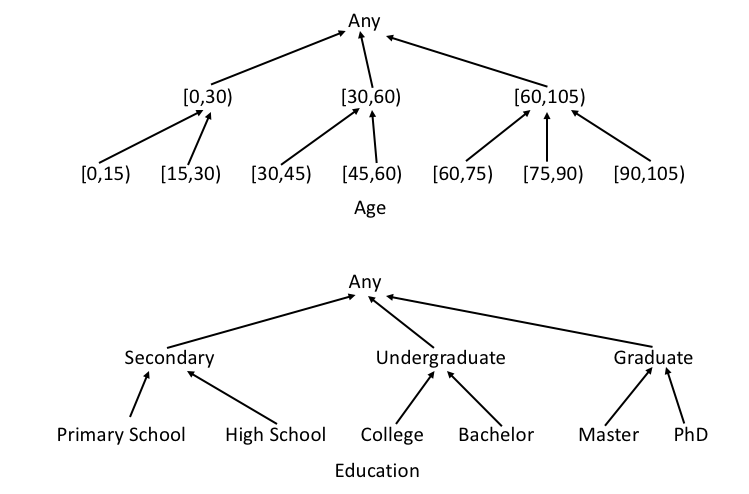
\includegraphics[scale=0.5]{Images/GenHier}
    \caption{Example generalization hierarchies}
    \label{fig:genhier}
\end{figure}

\noindent Note that this generalization approach is rather static and not data driven. The focus of this study is to provide an approach that is parallelizable and therefore scalable to high speed data streams. Furthermore, this static approach, as we will describe in detail later provides a guarantee for constant information loss, that is controllable and robust to outliers. With this setup we are able to leverage the functionality of Apache Flink in the best way.\\
\\
The novel approach that will be described in the following paragraphs is mainly based on \citeA{li2008} especially with respect to the generalization procedure, furthermore it makes use of some characteristics of the approaches of \citeA{CpppOfDataStreams}, but extends it by the $l$-diversity principle. Therefore, we will further introduce these algorithms and the differences to our approach at this point.\\
\\
Let's start with the algorithm of \citeA{li2008}: They introduce a data structure called the specialization tree. This tree is a combination of the generalization hierarchies (as described above) of the attributes in the quasi-identifier, where the root is the most general node. For a new arriving tuple, this specialization tree is scanned from the root until the most specific node is found, where the tuple fits in. Each node possesses a buffer, once a buffer satisfies $k$-anonymity, the tuples in the buffer are released and the node is marked as a work-node. The corresponding counterpart to the buffer in our approach is the window-functionality of Apache Flink, which will be described in detail later on. However, the main difference in the approach of \citeA{li2008} is that as soon as a node is marked as work-node, all arriving tuples at a work-node, will be released immediately. Note that this approach as a significant shortcoming. Assume an adversary registers that a certain equivalence class, that is, buffer of a node, was released and he knows the order or arrival time of tuples of that class arriving later, he would be able to infer the sensitive attribute of these tuples. In contrast, our approach will release tuples only in $k$-anonymous and $l$-diverse batches.\\
\\
\citeA{CpppOfDataStreams} adopt the same approach and only release $k$-anonymous batches of tuples. The main characteristic of the algorithms of \citeA{CpppOfDataStreams} is the data structure they use in order to group tuples to equivalence classes and generalize them, namely a R-Tree. Once a tuple arrives they insert the tuple into the R-Tree, therefore grouping similar tuples together into equivalence classes. The R-Tree is a dynamic index structure for multi-dimensional information and since it is dynamic, it is constantly reorganizing its nodes, which means that nodes are split at the insertion of new tuples, therefore always grouping tuples with the aim to minimize information loss \cite{guttman1984}. \citeA{CpppOfDataStreams} start with a randomized approach, where the probability that a equivalence class $C$, that is, a leaf node in the R-tree, is $Pr(C)=\frac{\beta}{loss(C)}$ to be published. The important thing to note is that the larger the information loss is, the smaller the probability for release is. On the other hand, $\beta$ indicates how long the leaf node stays in the R-Tree, that is the longer, the higher the probability of release. Subsequently, they introduce further measures and modifications to this algorithm in order to take into account the density distribution of attributes, or they hold tuples in dense areas to achieve higher anonymization quality. Basically the rationale behind this is that every split of leaf nodes in the R-tree leads to lower information loss, since it gets more granular. Therefore, if the distribution indicates that future tuples might lead to a split of leafs, it can be worth to wait until such tuples have arrived. Figure \ref{fig:cppp_result} illustrates the results for varying $k$. As can be seen, while certainly the anonymization security increases with $k$, so does the information loss in their approaches. This is the fact that we try to tackle in our approach by deploying a maybe simple generalization procedure, but at the same time being able to constrain information loss.

\begin{figure}[H]
    \centering
    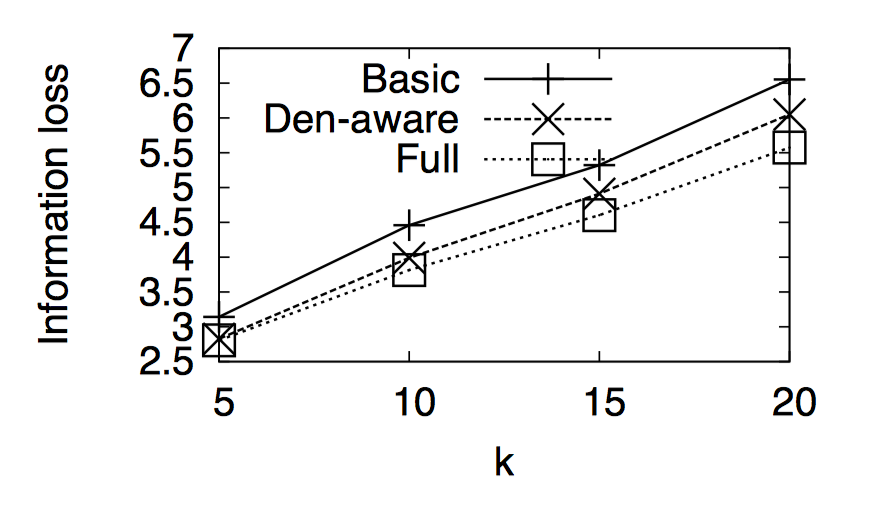
\includegraphics[scale=0.5]{Images/Cppp_k_anony_result.png}
    \caption{Information loss for different $k$ in the algorithms of Zhou et al. (2009)}
    \label{fig:cppp_result}
\end{figure}

\noindent Before we introduce the algorithm, let us clarify some notation: For a set $S$ of $j$ sensitive attributes, let $|S_m|$ denote the number of unique combinations of values for the $j$ attributes within some equivalence class $h$. For a tuple $t_i$ of the stream, let $g_i$ represent the generalized version of the tuple, which is retrieved by calling the function $generalize(t_i,QID)$, where $QID$ is the quasi-identifier set of attributes previously defined and with the corresponding generalization hierarchies. Furthermore, let $q_i$ be the values of the quasi-identifier for a tuple $t_i$ \textbf{after the generalization}, that is, these values are part of $g_i$. Lastly, let each $m \in $ $M$ be a collection of generalized tuples $g_i$, where each $g_i$ will be mapped to a collection $m$, with $q_i$ as mapping key. Each of the $m \in $ $M$  runs in one of $p$ distributed and parallel processes. Then the algorithm can be defined as below.

\noindent The most important characteristic of the algorithm that needs to be noted, is that the generalization of the tuples happens right when they arrive. This is only possible due to the nature of the static generalization, since one needs to be able to generalize single tuples. While this is a very restrictive necessity, it offers a number of advantages: 
1. Tuples are grouped by the generalization of the quasi-identifier, that ensures that only tuples are grouped together into an equivalence class which are very similar in their non-generalized version. This ensures robustness against outliers and therefore minimal information loss, given the quasi-identifier generalization. In the traditional approaches mentioned in the background section, the only criteria to group tuples together, is that they can't come from the same individual, this can lead to equivalence classes, that differ significantly in the values of the quasi identifier. However, these groups need to be generalized such that the tuples within such an equivalence class are indistinguishable. This can lead to a large information loss, to illustrate the problem consider for example two tuples one with Age 18 and another individual that has age 83, now if these two tuples are in the same equivalence class, it is impossible to find a generalization that preserves the information. The only way is to make very large interval, for example (15,85] or to replace the value by an asterisk "*". In comparison, since in our approach the tuples are grouped together only if they are very similar in their ungeneralized form and identical in their generalized form, this problem is prevented. Therefore, the approach is more robust to outliers and given a certain generalization, the information loss is minimal. 
2. The static generalization guarantees constant information loss, since no matter in which order or how the tuples arrive, they are always generalized in the same way, that is generalizing two identical tuples will always be generalized in the same way and with the same information loss. 
3. It enables us to distribute the process in a parallel way. The practical drawback of this approach, however, is that tuples with a less common quasi-identifier generalization will suffer from very long delays, even to the extent that the tuple can be considered as stuck. The number of tuples in the system at any given time has an upper bound induced by the number of unique possible combinations of the generalized quasi-identifier. In section 4 these potential advantages and drawbacks will be analyzed, and possible solutions discussed. 

\makeatletter
\def\BState{\State\hskip-\ALG@thistlm}
\makeatother

\floatname{algorithm}{Algorithm}
\renewcommand{\algorithmicrequire}{\textbf{\newline Input: }}
\renewcommand{\algorithmicensure}{\textbf{\newline Output: }}

\begin{algorithm}[H]
\caption{L-Diversity}\label{alg:ldiv}
\algorithmicrequire A stream $T$ of tuples to be anonymized, each tuple $t_i \in$ $T$, where $i$ is the arrival time and with a set of attributes $QID$, being the quasi-identifier and a set of $j$ sensitive attributes $S$. Parameters $k$, $l$ and $p$, where $p$ is the number of parallel processes. 
\algorithmicensure a stream $T'$ of $l$-diverse generalizations of $T$
\begin{algorithmic}[1]

\Procedure{L-Diversify}{$T, k, l, p$}
\newline
\textbf{Initialization}
\
\State Initialize $QID$ as a set of generalization hierarchies
\State Initialize set of collections $M = \emptyset$
\newline
\textbf{When a tuple $t_i \in$ $T$ arrives at instant $i$}
\
\State let $g_i$ := $generalize(t_i,QID)$ \Comment{Generalize the tuple}
\State retrieve $m \in M$ where $q_i$ maps to $m$ \Comment{Check if collection corresponding to $q_i$ exists}
\If{there is no such $m$}
\State create $m$
\EndIf
\State $m \gets g_i$ \Comment{Assign generalized tuple to collection}
\State assign $m$ to one of the $p$ parallel processes
\State $M \gets m$ \Comment{Put $m$ into the set $M$}
\If{$|m| > k$ \textbf{and} $|S_m| \geq l$} \Comment{If $m$ satisfies $k$-anonymity and $l$-diversity}
\State \textbf{release all $g \in m$ to output stream $T'$}
\State \textbf{remove $m_h$ from $M$}
\EndIf

\EndProcedure
\end{algorithmic}
\end{algorithm}

\newpage
\subsection{Solution architecture in Apache Flink}
This section serves to give a short description, of how the algorithm aligns with the functionality of Apache Flink and how the main parts have been implemented with the framework. 

\subsubsection{Data types}
 Given that the \textit{adult} data set from the UCI Machine Learning repository was used as a starting point of this study, the data is encapsulated in a class called \textit{AdultData} \cite{dua2017}. Figure \ref{fig:classdiagram} depicts class diagram of the data types that were implemented.\\ In later phases of the study the data set was replaced by a continuous data source that is creating tuples with the same value distributions as the original data set, in order to simulate longer streams and conduct the scalability and latency experiments in section 4.
 
 \begin{figure}[H]
    \centering
    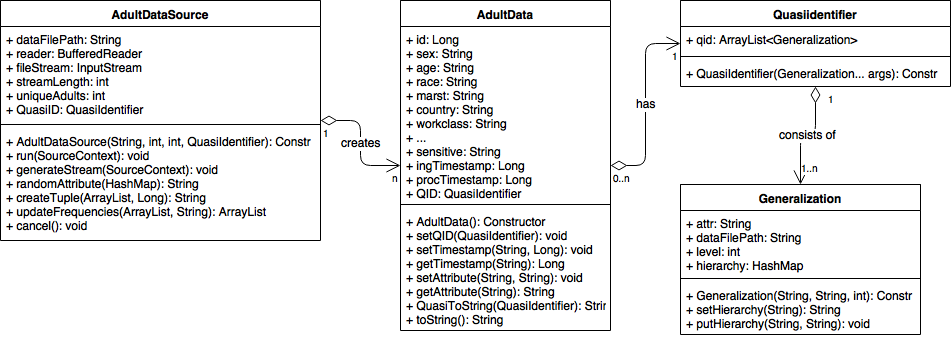
\includegraphics[scale=0.5]{Images/ClassDiagram.png}
    \caption{Class diagram of the implemented data types}
    \label{fig:classdiagram}
\end{figure}
 
 
\subsubsection{Logic and Class implementations}
\noindent  The core part of the implementation that ensures the parallelization of the algorithm is the piece of code in fig. \ref{fig:code}. Figure \ref{fig:flinkprocess} illustrates how the anonymization is implemented in Apache Flink. In this section we will comment on the code and usage of custom and Flink classes.  


\begin{table}[H]
\centering
\begin{tabular}{llll}

\toprule
Class & Extends/Implements & Functionality \\ \hline
KeyedJob & - & Main Class \\ 

AdultData & - & \multicolumn{2}{p{8cm}}{ A data type to contain the adult data tuples. }\\ 
AdultDataSource & SourceFunction & \multicolumn{2}{p{8cm}}{ Reads the adult data file, creates an extended stream of data. }\\ 


lDiversityTrigger & Trigger & \multicolumn{2}{p{8cm}}{ Asserts if a given GlobalWindow is \textit{K}-anonymous and \textit{L}-diverse, triggers Release process if so.}\\ 


Release & ProcessFunction & \multicolumn{2}{p{8cm}}{ When triggered, releases all AdultData objects in the triggered window. }\\ 
ProcessTimestamp & ProcessFunction & \multicolumn{2}{p{8cm}}{ Adds a time stamp to each element in a window. Is used to add ingestion time stamps to AdultData objects. }\\ 

Generalization & Serializable & \multicolumn{2}{p{8cm}}{ A data type to contain a generalization given a hierarchy and a generalization level.  }\\ 
QuasiIdentifier & Serializable & \multicolumn{2}{p{8cm}}{ A data type containing a Quasi Identifier consisting by several Generalizations  }\\ 
QidKey & KeySelector & \multicolumn{2}{p{8cm}}{ A function to return a key that will be used in the keyBy(), in this case the Quasi Identifier concatenated as a string.  }\\ 
Generalize & MapFunction & \multicolumn{2}{p{8cm}}{ Maps the ungeneralized value of the Quasi Identifier to the respective value in the generalization hierarchy. }\\ 




\bottomrule
\end{tabular}
\caption{Explanation of implemented classes}
\label{datacharac}
\end{table}


\begin{figure}[H]
    \begin{lstlisting}
    DataStream<AdultData> output = tsGenData
            .keyBy(new QidKey())
            .window(GlobalWindows.create())
            .trigger(lDiversityTrigger.of(k, l))
            .process(new Release());
            
    \end{lstlisting}
    \caption{Extract from KeyedJob.java}
    \label{fig:code}
\end{figure}

\noindent In the code executed in fig. \ref{fig:code}, a datastream is defined. First of all, the datastream is keyed by Quasi Identifier generalization through Flink's \textit{keyBy} function with the QidKey class as argument. Secondly, Flink's \textit{GlobalWindows} are used to keep track of the number of tuples in a key and the number of different sensitive values present in a equivalence class. Quoting Flink's documentation, a global window has the following characteristics: "A global windows assigner assigns all elements with the same key to the same single global window. This windowing scheme is only useful if you also specify a custom trigger. Otherwise, no computation will be performed, as the global window does not have a natural end at which we could process the aggregated elements." \cite{flink} Thirdly, the data stream is assigned a custom implemented trigger, \textit{lDiversityTrigger}, which asserts if a given \textit{GlobalWindow} is \textit{K}-anonymous and \textit{L}-diverse. Lastly, the data stream is assigned the \textit{Release} function which upon being triggered by the \textit{lDiversityTrigger} collects the tuples of a \textit{GlobalWindow} to the output stream. 

\begin{figure}[H]
    \centering
    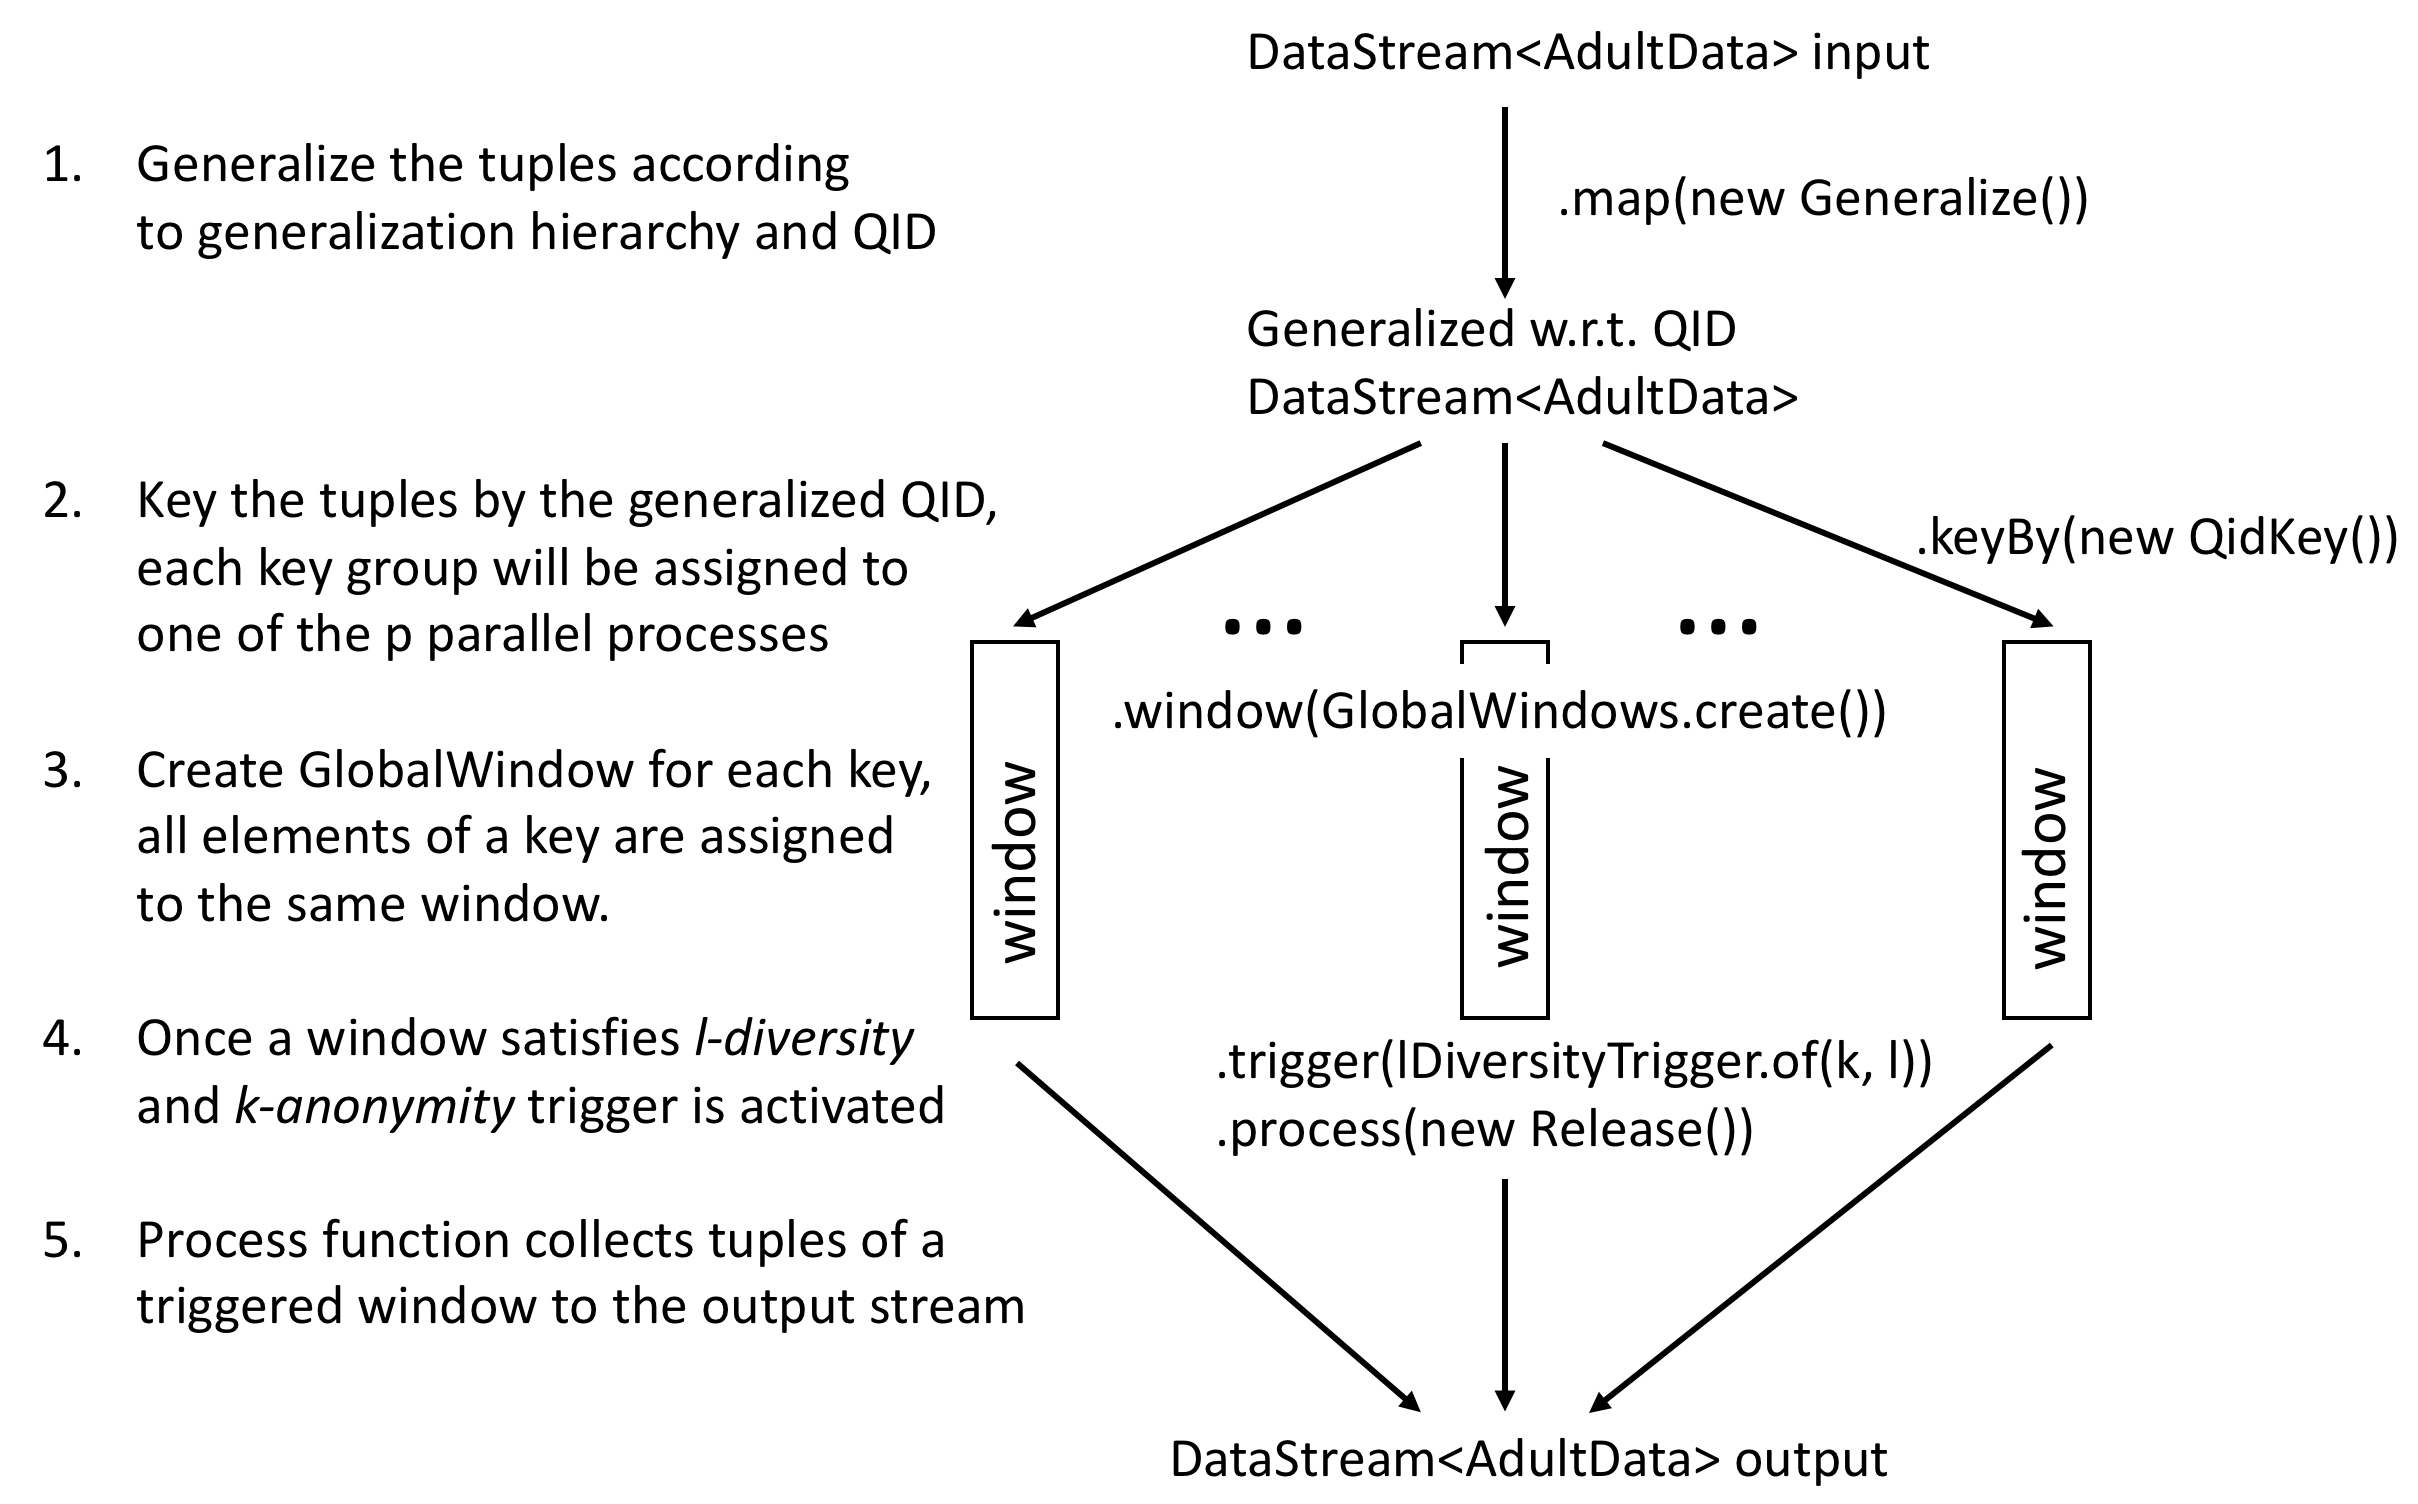
\includegraphics[scale=0.3]{Images/FlinkProcess_v2.png}
    \caption{Implementation in Apache Flink}
    \label{fig:flinkprocess}
\end{figure}
